\section{Large model}

We analyse the execution of large models on the GrAICore.
A large model is defined as a model with a size that is greater than the capacity of the GrAICore.
The main challenge for executing a large model is that it does not fit on the GrAICore as a single whole.

\subsection{Bandwidth analysis}
To target a specific input frame rate with a large model, we require information for the following components:
\begin{itemize}
    \item Number of model parts
    \item Configuration time for each model part. Which depends on:
    \begin{itemize}
        \item Write bandwidth
        \item Amount of data to write for each model part
    \end{itemize}
    \item Processing time for each model part
\end{itemize}

We approximate the maximum reachable input frame rate ($f$) as follows:
\begin{align*} 
    L &= \sum_{p \in P}^{}{p_{\textrm{config}} + p_{\textrm{process}}} \\
    f &= L^{-1}
\end{align*}

\begin{eqexpl}[15mm]
    \item{$L$} total latency
    \item{$P$} set of model parts
    \item{$p_{\textrm{config}}$} configuration time for model part $p$
    \item{$p_{\textrm{process}}$} processing time for model part $p$
    % \item{$f$} input frame rate
\end{eqexpl}

For example, assume we have a large model partitioned into four parts with each part requiring \SI{20}{MiB} to be written and has \SI{5}{ms} of processing latency.
The total latency is then only dependent on the available bandwidth, as it influences the configuration time:
\begin{equation*}
    % L = \left( \frac{\SI{20}{MiB}}{\textrm{BW}} + \SI{5}{ms} \right) \times 4
    f = \left[ \left( \frac{\SI{20}{MiB}}{\textrm{BW}} + \SI{5}{ms} \right) \times 4 \right]^{-1}
\end{equation*}

\begin{eqexpl}[15mm]
    \item{$\textrm{BW}$} available bandwidth
\end{eqexpl}

\begin{figure}
    \centering
        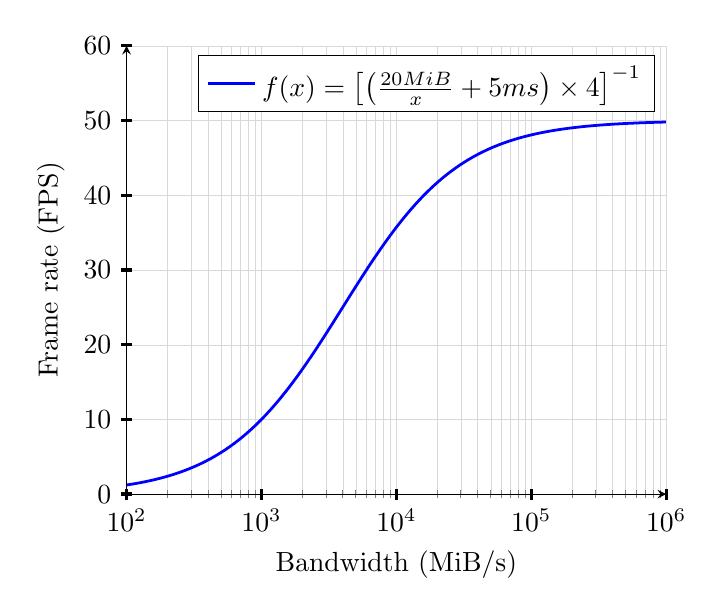
\begin{tikzpicture}
    \begin{semilogxaxis}[
        axis lines = left,
        xlabel = {Bandwidth (MiB/s)},
        ylabel = {Frame rate (FPS)},
        ymin = 0, ymax = 60,
        xmin = 100, xmax = 1000000,
        ytick distance=10,
        grid=both,
        grid style={line width=.1pt, draw=gray!30},
        every major tick/.append style={very thick, major tick length=4pt, black},
    ]
    
    \addplot [
        domain=1:1000000, 
        samples=1000, 
        color=blue,
        line width=1pt
    ]
    {1/((20/x + 0.005)*4)};
    
    \addlegendentry{$f(x) = \left[ \left( \frac{\SI{20}{MiB}}{x} + \SI{5}{ms} \right) \times 4 \right]^{-1}$}
    \end{semilogxaxis}
    \end{tikzpicture}

    \caption{Reachable frame rates with varying bandwidths for an example large model}
    \label{fig:large_model_bandwidth_analysis_example}
\end{figure}

\Cref{fig:large_model_bandwidth_analysis_example} shows that there is an horizontal asymptote at \SI{50}{FPS}\footnote{ $\lim_{x \to \infty} \left[ \left( \frac{\SI{20}{MiB}}{x} + \SI{5}{ms} \right) \times 4 \right]^{-1} = \SI{50}{Hz}$}.
Due to this, it is not possible to target an input frame rate of \SI{60}{FPS} for this model.
Even with an infinite write bandwidth, we can never reach \SI{60}{FPS}.
This limitation is due to the fixed processing latency of the four model parts (\SI{20}{ms}).
An input frame rate of \SI{30}{FPS} is possible and requires a write bandwidth of at least \SI{6}{GiB/s}.

With the bandwidth of the original config NoC (\SI{763}{MiB/s}), we can target up to \SI{8}{FPS}\footnote{$\left[ \left( \frac{\SI{20}{MiB}}{\SI{763}{MiB/s}} + \SI{5}{ms} \right) \times 4 \right]^{-1} \approx \SI{8}{Hz}$}.
 
\section{Execution of the ResNet-101 model}
\todo[inline]{Move this to separate section? \cref{section:tmp}}

We will be looking at the execution of a large model on the GrAICore.
In particular we will be using a specific model as an example throughout this subsection.

The ResNet-101 model is a deep neural network commonly used for computer vision applications \cite{heDeepResidualLearning2015}.
We will be using the ResNet-101 model from the \textit{Keras} library \cite{KerasDocumentationResNet} pretrained on the ImageNet database \cite{russakovskyImageNetLargeScale2014}
The ResNet-101 model has around \SI{44.5}{M} parameters in total.
An important feature of the ResNet architecture is the use of skip connections \cref{TODO}.

Due to the size (amount of parameters) of the ResNet-101 model, it is not possible to load the model on the GrAICore at once.
This is still the case when representing the parameters with low-precision data types like 8-bit integers or floats (this also known as quantization).
Other solutions, such as model compression techniques exist to decrease the size of the model.
However, as explained earlier, this has its disadvantages such as decreased inference accuracy.

To allow the model to fit on the GrAICore we will be looking at partitioning the model into smaller parts.
A model part is capable of being (completely) loaded on the GrAICore.
By sequentially loading and processing each of the model parts, the full functionality of the original (large) model can be emulated.
The output data of each model part must be buffered outside the local memories, and will be used as input for the subsequent model part.
The amount of data to be buffered is dependent on the output shape of the final layer of a part.

% Due to ResNet's extensive use of skip connections, it is not straightforward to split/partition the model at any location. We therefore only consider locations in the network where it is easy to split. In most cases this is at locations right before or after a split connection.

\begin{figure}[hbtp]
    \centering
    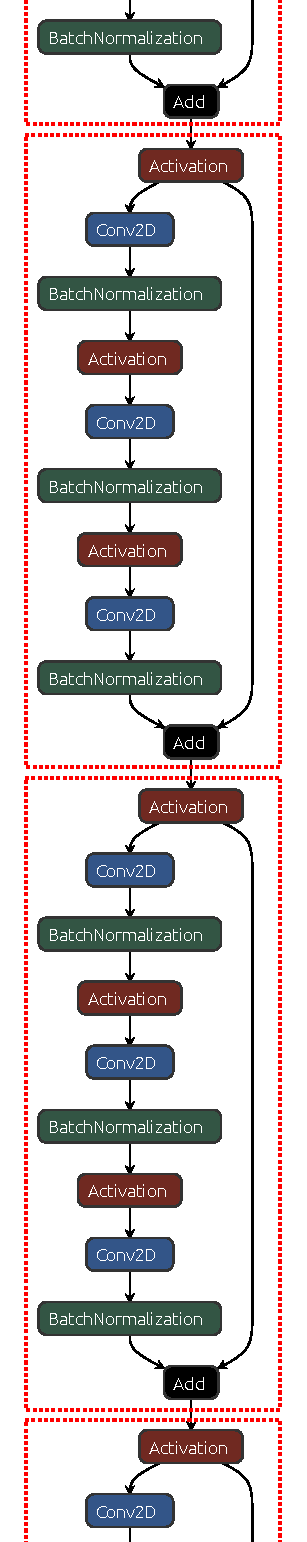
\includegraphics[angle=90, width=\linewidth]{assets/resnet101_residual_blocks.pdf}
    \caption{
    Snippet of a visualization of the ResNet-101 network.
    The red rectangles represent the residual blocks.
    }
    \label{fig:resnet101_residual_blocks}
\end{figure}

The ResNet architecture introduces so-called residual blocks (see \cref{fig:resnet101_residual_blocks}).
A residual block contains a collection of layers with a special type of connection from the beginning of the block until the end of the block.
This connection is also called a skip connection.
Due to these skip connections, it is not straightforward to split the ResNet-101 model at any location.
Splitting the model between two layers where also a skip connection resides, will introduce a few difficulties.
Firstly, you will require to buffer multiple outputs.
That is, the output data of the layer just before the split point and the output data of the skip connection.
Secondly, the two outputs need to be propagated to their respective destination layers.
These two outputs can have the same or different destination layer.
If they have different destinations, the output of the skip connection needs to be buffered until the network reaches a later stage.

In the context of the GrAICore, this adds challenges to the system.
Not only does this increase the instantaneous total memory usage, it also increases the energy usage.
More energy is consumed due to the increased data to be buffered.
This is especially evident due to the need to buffer the data on some external memory.
Next to this buffering problem, software support must also be provided.
The current system only allows for a single input to the model. 

Due to these complexities, we keep the partitioning of the ResNet-101 model simple and only consider partitioning the network at locations where no skip connections appear.
Naturally, the main drawback of this is the reduces number of locations where partitioning can occur.

\begin{figure}[hbtp]
    \centering
    \subcaptionbox{MACs per residual block \label{fig:resnet101_macs}}[\textwidth]{
        \pgfplotstableread[col sep=semicolon]{assets/resnet101_stats.csv}\datatable
\begin{tikzpicture}
    \begin{axis}[
        width=\textwidth,    % set width
        height=0.3\textwidth, % and height
        ybar,
        enlarge x limits={rel=0.05},
        bar width=8pt,   % they were too wide
        xlabel={Residual block},
        ylabel={MACs},
        xlabel style={yshift=-1em},
        xtick=data,
        xticklabel style={rotate=45, font=\scriptsize, anchor=east},
        xticklabels from table={\datatable}{index},
    ]
    \addplot table[x expr=\coordindex, y={macs}]{\datatable};
    \end{axis}
\end{tikzpicture}

    }
    \subcaptionbox{Number of parameters per residual block \label{fig:resnet101_params}}[\textwidth]{
        \pgfplotstableread[col sep=semicolon]{assets/resnet101_stats.csv}\datatable
\begin{tikzpicture}
    \begin{axis}[
        width=\textwidth,    % set width
        height=0.3\textwidth, % and height
        ybar,
        enlarge x limits={rel=0.05},
        bar width=8pt,   % they were too wide
        xlabel={Residual block},
        ylabel={\# Parameters},
        xlabel style={yshift=-1em},
        xtick=data,
        xticklabel style={rotate=45, font=\scriptsize, anchor=east},
        xticklabels from table={\datatable}{index},
    ]
    \addplot table[x expr=\coordindex, y={params}]{\datatable};
    \end{axis}
\end{tikzpicture}
    }
    \caption{
        MACs and the number of parameters per residual block.
        The tuple $(x, y)$ represents the residual block at index $y$ of the stage at index $x$.
        \textit{Head} and \textit{tail} contain the remaining layers at the start and end of the network respectively.
    }
    \label{fig:resnet101_stats}
\end{figure}

The ResNet-101 model contains five so-called stages.
A stage is a collection of consecutive layers.
Only the first stage does not include any residual blocks.
The other stages contain different amounts of residual blocks as shown in \cref{fig:resnet101_stats}.

If we opt to split the network based on computational complexity, we look at the amount of multiply-accumulate (MAC) operations of the layers.
A MAC operation is essentially a multiplication operation followed by a addition operation.
Since we only perform splits between residual blocks, we combine the MACs of each layer in the residual blocks.
In \cref{fig:resnet101_macs}, we observe that the amount of MACs for each residual block is relatively similar.
We see small peaks at the start of each stage.
This is due to an additional convolution layer in the first residual block of a stage.
% A model or model part with more MACs generally is more heavy to run than those with less MACs (lower .
Generally, a model or model part with high number of MACs take longer to process fully.

In \cref{fig:resnet101_params}, we observe that the distribution of the parameters do vary significantly over the residual blocks.
The graph shows that the last few residual blocks carry a significant portion of the total parameters.
Again, we see small peaks at the start of each stage.
Naturally, a model part with a higher number of parameters will require more memory space.
Due to the uneven distribution of the parameters we have less flexibility with partitioning. 

\section{Splitting}
The ResNet-101 model has a total parameter count of around \SI{44.5}{M}.
Even if the parameters are quantized to an 8-bit datatype, the model will still not fit on the GrAICore as a whole.
Weights stored on the GrAICore require one extra bit.
% This extra bit is used as a mask that activates or deactivates the associated weight.
This extra bit is used to indicate whether a weight is removed (i.e., pruned) or not.
However, since we are using the original ResNet-101, no pruning has been applied to the weights.
We can roughly say that the network requires \SI{47.7}{MiB}\footnote{$\frac{\num{44496488} \times 9}{8} \times \frac{1}{2^{20}}$} of memory capacity for the parameters when quantized to 8 bits.
However, this does not include any mandatory header information and buffer space when mapping the network for the GrAICore. 

The in-house compiler for the GrAICore is complex and we will not get into detail.
In a nutshell, the compiler first optimizes the model by converting it to a so-called \textit{GrAI Model}.
Among other things, the optimized model slightly changes the architecture of the network and optionally performs post-training quantization \cref{TODO} for the weights.
The amount of MACs and parameters stay roughly the same.
Afterwards, it will map the layers of the model to the neuron cores.
The compiler can be instructed to optimize for inference latency.
This is done, for example, by mapping a single layer to multiple neuron cores to exploit parallelism.

Splitting the network between the residual blocks $(4, 18)$ and $(4, 19)$, we obtain two parts with roughly the same number of parameters (\SI{21.9}{M} and \SI{22.6}{M}).
For the weights, this is \SI{23.5}{MiB} and \SI{24.2}{MiB} respectively.

\hrulefill


\subsubsection{ResNet-101 partitioned in 5 parts}
One example partitioning is done as follows (note that the parameters are quantized to 8 bits).
The ResNet-101 model is partitioned in 5 parts.
The compiler is able to compile each of the parts, indicating that they are configurable on the GrAICore.
The processing latency for each of the parts can be estimated by using the in-house GrAIPEFRUIT simulator.
Furthermore, the compiler also provides us information about how much data must be written to each of the neuron cores.
Note that the compiler can map a layer to multiple neuron cores.
This requires the weights to be written to all neuron cores that require them.
This means that the GrAICore contains duplicate weights.
The total data to write and processing latency for each part is shown in \cref{tab:resnet101_5parts}.

\begin{table}[hbtp]
\centering
\begin{tabular}{@{}llll@{}}
\toprule
\textbf{Part}  & \textbf{To write (MiB)} & \textbf{Latency (ms)} & \textbf{Time to configure (ms)} \\ \midrule
1              & 28.75                   & 7.08                  & 2.36                            \\
2              & 20.06                   & 2.65                  & 1.64                            \\
3              & 30.44                   & 4.01                  & 2.49                            \\
4              & 17.71                   & 2.34                  & 1.45                            \\
5              & 15.54                   & 2.04                  & 1.27                            \\ \midrule
\textbf{Total} & 112.51                  & 18.12                 & 9.22                            \\ \bottomrule
\end{tabular}
\caption{Statistics of the ResNet-101 model partitioned in 5 parts}
\label{tab:resnet101_5parts}
\end{table}
% Using the proposed config NoC, we can reach a peak write bandwidth of 11.92 GB/s.
With the write bandwidth of the newly proposed config NoC (\SI{11.92}{GiB/s}), we compute the time to configure each of the parts (see \cref{tab:resnet101_5parts}).
The sum of the configuration times and processing latencies is \SI{27.34}{ms}.
This means that we can (at best) process frames with an input frame rate of \SI{36.6}{FPS}\footnote{$\frac{1}{\SI{27.34}{ms}}$}.
% The compiler accepts many parameters that can affect the performance (e.g., inference latency or power usage) when the model is running on the GrAICore.

% However, before mapping this network to the GrAICore, the model needs to be converted to a new model optimized for the GrAICore called GrAIModel. Among other things, the optimized model slightly changes the architecture of the network and performs quantization for the weights (if this was chosen). We observe that the MACs stay roughly the same while the number of parameters do change.

% When compiling the network/model for the GrAICore, it firstly gets converted to a GrAIModel. Afterwards, it will map the layers to the neuron cores. For improving the inference latency, it can map (parts of) a single layer to multiple neuron cores to exploit parallelism.

% The compiler for the GrAICore is complex and we will not get into detail. In a nutshell, the compiler optimizes the input model to a GrAIModel, afterwards it will map the layers to the neuron cores. It can optimize for inference latency by exploiting parallelism. This is done by, for example, mapping a single layer to multiple neuron cores.


%%%

% There are many ways to partition a model. 
% Amount of parts (there is a minimum)
% Distribution of parameters
% Distribution of FLOPS/MACs

% We use the in-house compiler to find a valid mapping for the GrAICore, with focus on low processing latency. The compiler also outputs files necessary for simulating the networks with GRAIPEFRUIT. GRAIPEFRUIT is used to approximate the processing latency of a network.
% Note that the compiler is a complex piece of software. Since it accepts many parameters, it is difficult to find an optimal mapping. 
